\documentclass[11pt, t,aspectratio=169]{beamer}
%\documentclass[11pt, t,aspectratio=169,handout]{beamer}

% additional options: german, unilogo, guestlogo, department, depunilogo
\usepackage{style/beamerthemeipvs}

%\usepackage{lmodern} %new font-shapes
\usepackage{amsmath}
\usepackage{amssymb}
\usepackage{amsthm}
\usepackage{colortbl}
\usepackage{multicol}
\usepackage{dsfont}
\usepackage{tikz}
\usepackage[format=hang]{subfig}
%\usepackage{subfigure}
\usepackage{esvect}
% pseudo-code
\usepackage{algorithm} 
\usepackage{algpseudocode} 
\usepackage{tabularx}
\newcommand{\algorithmautorefname}{Algorithmus}
\usetikzlibrary{positioning}

% calligraphic
\newcommand{\cA}{\mathcal{A}}
\newcommand{\cB}{\mathcal{B}}
\newcommand{\cC}{\mathcal{C}}
\newcommand{\cD}{\mathcal{D}}
\newcommand{\cE}{\mathcal{E}}
\newcommand{\cF}{\mathcal{F}}
\newcommand{\cG}{\mathcal{G}}
\newcommand{\cH}{\mathcal{H}}
\newcommand{\cI}{\mathcal{I}}
\newcommand{\cJ}{\mathcal{J}}
\newcommand{\cK}{\mathcal{K}}
\newcommand{\cL}{\mathcal{L}}
\newcommand{\cM}{\mathcal{M}}
\newcommand{\cN}{\mathcal{N}}
\renewcommand{\O}{\mathcal{O}}
\newcommand{\cP}{\mathcal{P}}
\newcommand{\cQ}{\mathcal{Q}}
\newcommand{\cR}{\mathcal{R}}
\newcommand{\cS}{\mathcal{S}}
\newcommand{\cT}{\mathcal{T}}
\newcommand{\cU}{\mathcal{U}}
\newcommand{\cV}{\mathcal{V}}
\newcommand{\cW}{\mathcal{W}}
\newcommand{\cX}{\mathcal{X}}
\newcommand{\cY}{\mathcal{Y}}
\newcommand{\cZ}{\mathcal{Z}}


\newcommand{\D}{\ensuremath{\mathcal{D}}}

% greek
\newcommand{\ga}{\alpha}
\newcommand{\gb}{\beta}
\newcommand{\gd}{\delta}
\newcommand{\gf}{\phi}
\renewcommand{\gg}{\gamma}
\newcommand{\gk}{\kappa}
\newcommand{\gl}{\lambda}
\newcommand{\go}{\omega}
\newcommand{\gs}{\sigma}
\newcommand{\gt}{\theta}
\newcommand{\gz}{\zeta}
\newcommand{\vp}{\varphi}
\newcommand{\vt}{\vartheta}
\newcommand{\gD}{\Delta}
\newcommand{\gG}{\Gamma}
\newcommand{\gL}{\Lambda}
\newcommand{\gO}{\Omega}
\newcommand{\gP}{\Phi}
\newcommand{\gT}{\Theta}

%Def's by ab
\newcommand{\R}{\mathds{R}}
\newcommand{\N}{\mathds{N}}
\newcommand{\T}{\mathds{T}}
\newcommand{\bP}{\mathds{P}}
\newcommand{\ind}{\text{IND}}
\newcommand{\cat}{\text{CAT}}
\newcommand{\cdd}{\text{CDD}}
\newcommand{\hdd}{\text{HDD}}
\newcommand{\var}{\text{Var}}
\newcommand{\cov}{\text{Cov}}
\newcommand{\abs}[1]{\left\vert#1\right\vert}
\newcommand{\Op}{\operatorname{O}}
\newcommand*{\lrscript}[5]{{\vphantom{#1}}_{#2}^{#3}{#1}_{#4}^{#5}}
\newcommand*{\dualpair}[4]{\ensuremath{\lrscript{\langle}{#1}{}{}{} #3 ,
#4 \rangle_{#2}}}
\newcommand{\KL}{{Karh\'{u}nen-Lo\`{e}ve }}
\newcommand*{\hV}{\ensuremath{\hat{V}}}


%\numberwithin{Theorem}{section}
\newcommand{\IR}{{\mathbb R}}
\newcommand{\IN}{{\mathbb N}}
\newcommand{\IT}{{\mathbb T}}
\newcommand{\dis}{\displaystyle}
\newcommand{\n}{\noindent}
\newcommand{\hs}{\hspace{-1ex}}
\newcommand{\matr}[1]{\boldsymbol#1}
\newcommand{\dsl}{\displaystyle\sum\limits}

\newcommand{\ba}{\begin{eqnarray}}
\newcommand{\ea}{\end{eqnarray}}
\newcommand{\esp}{\mathbb{E}}
\newcommand{\E}{\mathds{E}}
%\newcommand{\R}{\mathds{R}}
%\newcommand{\N}{\mathds{N}}
\newcommand{\IP}{\mathds{P}}
\newcommand{\IF}{\mathds{F}}
%\newcommand{\cF}{\mathcal{F}}
%\newcommand{\cB}{\mathcal{B}}
%\newcommand{\cG}{\mathcal{G}}
%\newcommand{\cN}{\mathcal{N}}
\def\e{{\text{e}}}

%\newcommand{\norm}[1]{\| #1 \|}
\newcommand{\inprod}[2]{\langle #1,#2 \rangle}
\renewcommand{\vec}{\underline}
\def\ci{\perp\!\!\!\perp}

%\usepackage{color}
\newcommand{\cred}{\color{red}}
\newcommand{\cblue}{\color{blue}}
\newcommand{\cblack}{\color{black}}
\newcommand{\cgreen}{\color{green}}
\definecolor{bluefromheader}{cmyk}{.83,.44,0,.33} 
\newcommand{\dc}{\color{bluefromheader}}
\newcommand{\as}{\textcolor{red}}


\newcommand\norm[1]{\lVert#1\rVert}
\renewcommand\qed{$\hfill\square$}
\newcommand\scprod[2]{\langle #1 , #2 \rangle}
\definecolor{boxcolor}{RGB}{187, 222, 232}


\usepackage[backend=biber]{biblatex}
\bibliography{../bib/literatur.bib}

%%%%%%%%%%%%%%%%%%%%%%%%%%%%%%%%%%%%%%%%%%%%%%%%%%%%%%%%%%%%%%%%

\title{Towards Real-Time Physics in a 2D Survival-Based Game}
%\subtitle{oder warum der direkte Weg manchmal zu lang ist}
\author[B. Aheimer, F. R\"ohr, D. Six, A. Vezenkov, A. Weckauff]{\vspace{-.25cm}\footnotesize{B. Aheimer,\\F. R\"ohr,\\D. Six,\\A. Vezenkov,\\A. Weckauff}}
\date{18. November 2024}
\institute{IPVS/SGS}
\pgfdeclareimage[width=2.5cm]{speaker}{../../assets/texture/duck.png} % speaker photo for final slide
\pgfdeclareimage[width=2.5cm]{department}{logos/logo_simtech.pdf}
\pgfdeclareimage[width=2.5cm]{thanksto1}{thanks/thanks1}
\pgfdeclareimage[width=2.5cm]{thanksto2}{thanks/thanks2}
\pgfdeclareimage[width=2.5cm]{thanksto3}{thanks/thanks3}
\pgfdeclareimage[width=2.5cm]{thanksto4}{thanks/thanks4}

%%%%%%%%%%%%%%%%%%%%%%%%%%%%%%%%%%%%%%%%%%%%%%%%%%%%%%%%%%%%%%%% 

% individual picture on front page
\setTitlepic{\includegraphics{../figures/new_game.png}}
 %\setTitlepic{\hspace*{-2cm}\includegraphics[height=3cm]{f8banner}}

% Logo subtext on frontpage (uncomment for Germany-Subtext with english logo)
\setLogoText{Bachelor Research Project Computer Science}

%%%%%%%%%%%%%%%%%%%%%%%%%%%%%%%%%%%%%%%%%%%%%%%%%%%%%%%%%%%%%%%%

\begin{document}
	
	\begin{frame}[plain]
		\titlepage
	\end{frame}

	\IEEEraisesectionheading{\section{Introduction}\label{sec:introduction}}
\nocite{ProjectCode}
The objective of the project \glqq Towards real-time physics in a 2D survival-based game\grqq{} is
a comprehensive restructuring and improvement of the original game \glqq Surviving Sarntal\grqq{}.
This comprises three major work packages: software engineering, development of real-time physics and game engineering.

% Software engineering part: 
The first part of the project focuses on improving the code by adherence to software engineering principles.
This includes extensive refactoring of the original code base, designing a new and maintainable software architecture,
establishing protocols for development, testing and clean code as well as creating a platform for detailed documentation for users and developers.
The project's continuous progress was ensured by applying Scrum principles and structuring it in sprints \cite{scrum}.
% We carried out a total of three sprints, whereby at the beginning of each sprint we defined the objectives at the end of the sprint
% and the issues to be dealt with. On a weekly basis, a meeting was held with our supervisor.
% During these meetings, the current progress regarding the project timeline, ideas and challenges occurring in development were discussed.
% Furthermore, two time slots were determined each week for a brief discussion of each team member's current work.
% The GitLab \glqq Issues\grqq{} were used to determine feasible work packages, which then could be assigned to one team member.

% Real time physics: 
The primary goal of the development phase is the enhancement of the real-time physics,
which involves the implementation of realistic 2D physics without compromising real-time performance.
This was accomplished by decoupling the physics simulation rate from the frame rate.
Furthermore, the project includes the development and implementation of improved models and algorithms
for interaction between game elements such as collision detection and handling.

% Game engineering
Moreover, the project contributes to the enhancement of the game design as a whole.
A number of new elements have been implemented, such as configurable 2D spline-based terrain generation, 
new items with improved functionality, new rock generation, increasing difficulty and updated audio and graphics.

% "Conclusion of the Introduction" 
In essence, the project was developed in accordance with the vision of creating an enhanced version of the game \glqq Surviving Sarntal\grqq{}
that would offer users a realistic physics simulation, engaging gameplay, and aesthetically pleasing visuals as well as creating a maintainable code base.
The code for the game is available as a git repository here \cite{ProjectCode} and it is open source under an MIT license.

\subsection{The Game}
The general goal of the game is for the hiker to survive as long as possible and climb as high as possible. 
The player is chased by a monster and needs to evade rocks that roll down the mountain. 
Moreover, the player may collect items that give the hiker additional benefits like restoring health and adding a protective shield. 
A comprehensive guide to the controls can be found in the project documentation \cite{ProjectWiki} and at the start of the game under the menu "Instructions". 

\subsection{Transformation of the original game}
The original game \glqq Surviving Sarntal\grqq{} was created within a few days at the \glqq Ferienakademie 2023\grqq{}.
In this project, we refactor the original game in a significant way. 

\subsubsection{ECS vs. OOP}
The original game is based on the Entity-Component-System (ECS) framework flecs \cite{flecs_library}.
As a team, we decided to alter the project's fundamental architecture by shifting from ECS
to an object-oriented programming (OOP) approach.
Given our familiarity with OOP, we came to the conclusion that transitioning from ECS to OOP
would allow us to create a code base that could be easily comprehended, expanded and maintained.

\subsubsection{Transformation of Graphics}
During the development process of the new version of the game, we decided that a complete rework of the game's graphics was necessary.
New and creative graphical elements were created for all aspects of the game, including the entities, terrain, and background, and were integrated into the rendering phase of the game.
Screenshots of the old game can be seen in fig. \ref{fig:old_game} and of the new game in fig. \ref{fig:new_game}.

\begin{figure}[h!]
    \centering
    \includegraphics[width=0.45\textwidth]{figures/old_game.jpeg}
    \caption{Screenshot of the original game graphics.}
    \label{fig:old_game}
  \end{figure}

\begin{figure}[h!]
    \centering
    \includegraphics[width=0.45\textwidth]{figures/new_game.png}
    \caption{Screenshot of the renewed game graphics.}
    \label{fig:new_game}
  \end{figure}

\subsubsection{Addition of a game menu}
As a new feature we include a game menu.
A start menu is shown once the game has been initiated, which allows the user to access instructions and controls, and to start the gameplay.
An end screen appears after the hiker has died, which enables them to start another round of gameplay. 
We also add a pause screen, which gives the user the options to go back to the main menu or continue the game.

\subsubsection{Modular Architecture}
As part of the software engineering work package of the project we designed a modular game architecture that provides several key benefits:
\begin{itemize}
    \item \textbf{Ease of Maintenance:} Since components such as rendering, physics, and spawning are isolated from each other, it is easier to modify, debug, or upgrade parts of the game without introducing side effects.
    \item \textbf{Maintainability:} New features or game elements (e.g., new items, enemies, or gameplay mechanics) can be added by extending existing systems without requiring significant changes to the core architecture.
    \item \textbf{Testing and Debugging:} We add multiple features for developers, like a debug view seen in fig. \ref{fig:debug_mode} and a developer mode of the game that allows the running of predefined test cases. 
    \item \textbf{New terrain:} We extend our modular design to the terrain, by creating a completely new class structure that allows for different terrains with different features to be added.
\end{itemize}
This modular structure enables the development team to build complex systems in a more controlled and efficient manner, leading to a highly extensible and maintainable game.


	\makesection{Game}

\begin{frame}{The Game Concept}
    \begin{itemize}
        \item Endless runner game focused on survival.
        \item Player controls a hiker who must dodge rocks and survive as long as possible.
        \item Collect items along the way to gain health, protection, or other benefits.
    \end{itemize}
\end{frame}

\begin{frame}{The Game Concept}
    \begin{itemize}
        \item Endless runner game focused on survival.
        \item Player controls a hiker who must dodge rocks and survive as long as possible.
        \item Collect items along the way to gain health, protection, or other benefits.
    \end{itemize}
\end{frame}
	\section{Game Architecture}

%\begin{figure*}[!t]
%    \centering
%    \includegraphics[scale=0.25]{figures/Architectural-Diagramm.drawio.png}
%    \caption{Architectural diagram}
%    \label{fig:architecture}
%\end{figure*}

The game is built using a highly modular architecture that allows for flexibility, scalability, and ease of maintenance.
The modular design breaks down the game into distinct components, each responsible for a specific functionality.
This approach ensures that different parts of the game can be developed, tested, and modified independently, making the overall system more manageable.
Below, we describe the general architecture and how different parts contribute to building the game.

\subsection{The Game Loop}\label{sec:gameLoop}

The game loop is the central control unit of our program and defines the interaction of the game's core components.
It contains all the logic and data needed to run the actual gameplay.
Our game loop is depicted in fig. \ref{fig:gameLoop}.
For the most part, it adheres to the industry standard as described by Nystrom \cite{nystromGameLoop} and the Unity framework \cite{unityGameLoop}.
Hence, we will only briefly describe its functionality here.

\begin{figure}[h!]
    \centering
    \includegraphics[width=\linewidth]{figures/physics/gameLoop.pdf}
    \caption{The game loop represents the fundamental structure of the game and comprises three distinct phases. The terrain generation is performed concurrently.}
    \label{fig:gameLoop}
\end{figure}

At the start of the game loop, input from the player, be it via keyboard or gamepad, is registered and passed to the physics engine.
The physics engine progresses the simulation in one or more constant time steps between frames (c.f. decoupling in sec. \ref{sec:decoupling}), thereby processing the collected input events.
Finally, the renderer draws the new frame representing the updated world state.

Due to the sequential nature of input receipt, input processing, simulating a physics step, and rendering the resulting new state of the world, the game loop is also inherently sequential.
For very large games or powerful frameworks such as the aforementioned Unity framework, a parallelization becomes inevitable, but in our game, this structure suffices.
As described in sec. \ref{sec:performance}, the physics engine does not have to run on a separate thread for our purpose.
Merely the terrain generation is extracted from the spawning phase of the physics engine in order to guarantee a smooth transition between biomes during gameplay.

\subsection{Core Components and Services}

The game is initialized through a \code{GameFactory} class, responsible for building and configuring all core components and dependencies.
These components can be categorized into services, game entities, menu systems, rendering pipelines, spawning systems, and the physics engine.

\subsection{Services}
Several core services are initialized within the \code{GameFactory} to manage resources, input, and audio:

\begin{itemize}
    \item \textbf{ConfigService:} A singleton pattern is used to handle game configuration (including YAML settings), ensuring game constants and configurations are readily available throughout the game.
    \item \textbf{InputService:} A singleton service responsible for managing input from various devices, such as gamepads and keyboards.
    \item \textbf{ResourceService:} Handles loading and management of game assets such as textures, audio, and other resources. It depends on the \code{ConfigManager} to load the assets specified in the YAML file.
    \item \textbf{AudioService:} Manages sound effects and background music. It interacts with the \code{ResourceManager} to load sound files and handle audio playback within the game.
    \item \textbf{DifficultyService:} A singleton service that manages the difficulty progression during the gameplay.
\end{itemize}

\subsection{Game Entities}

Key in-game entities, such as the terrain, hiker, and inventory, are created and managed by the \code{GameFactory}.
These entities interact with the world and with each other, providing the core gameplay functionality.

\begin{itemize}
    \item \textbf{Terrain:} Generated based on game constants and managed by the \code{Terrain} class. It determines the physical environment in which the player interacts.
    \item \textbf{Hiker:} The main player character, represented by the \code{Hiker} class.
    \item \textbf{Monster:} An antagonist entity represented by the \code{Monster} class, which adds an element of challenge for the player, acting as a threat.
    \item \textbf{Inventory:} Manages the player's items and inventory.
\end{itemize}

These entities are bound together within the \code{World} class, which encapsulates the terrain, hiker, monster, and inventory, managing their interactions.


\subsection{Spawner System}

The game includes a system for dynamically spawning items and rocks during gameplay:

\begin{itemize}
    \item \textbf{ItemSpawner:} Spawns items in the world based on configuration from the YAML file (e.g., item spawn rates and types).
    \item \textbf{RockSpawner:} Dynamically spawns rocks of various sizes, speeds, and densities during gameplay, adding an element of challenge.
    \item \textbf{Spawner:} A unified spawner that manages both the \code{ItemSpawner} and \code{RockSpawner}. It also initiates the terrain generation.
\end{itemize}

This modular spawner system allows for dynamic game elements that can evolve based on player progress or difficulty.
\pagebreak
\subsection{Physics and Collision Detection}

The game incorporates a robust physics engine to handle movement, collisions, and interactions between entities:

\begin{itemize}
    \item \textbf{Accelerator:} Applies acceleration forces to the entities to the hiker and other objects in the game world. So far, only gravitational forces are considered.
    \item \textbf{CollisionDetector:} Detects collisions between entities (e.g., hiker and terrain, rocks, or inventory items) to trigger corresponding responses.
    \item \textbf{CollisionHandler:} Handles the game logic triggered by collisions, such as taking damage or picking up items.
    \item \textbf{Destructor:} Handles the accurate and timely destruction of entities.
    \item \textbf{Positioner:} Handles the correct positioning of the entities within the game
    \item \textbf{PhysicsEngine:} The central physics engine that manages all other physics modules.
\end{itemize}
By abstracting collision detection and handling into separate classes, the game ensures that its physics are flexible and can easily be adapted or expanded upon.

\subsection{Menus and UI}

The game uses a sophisticated menu system to handle the user interface, including in-game menus. This system is composed of:

\begin{itemize}
    \item \textbf{MenuEngine:} Responsible for managing the game's various menus, including the start screen, settings, and pause menus. It also handles user input in these menus.
    \item \textbf{FullMenuRenderer:} Renders the menu components on the screen.
    \item \textbf{MenuEventProcessor:} Handles events that occur within the menus, such as button clicks and navigation.
\end{itemize}

This system ensures that the menu and UI are distinct from the core game logic, allowing independent development and modification of the user interface.

\subsection{Renderer}

The game rendering is divided into several subsystems to ensure modular and efficient drawing of different elements:

\begin{itemize}
    \item \textbf{PolygonRenderer:} Used for drawing polygonal shapes, typically for terrain or other geometric elements.
    \item \textbf{MountainRenderer:} A specialized renderer for drawing the mountain and environmental elements in the background.
    \item \textbf{EntityRenderer:} Handles rendering of game entities (e.g., the hiker, inventory items, and the monster).
    \item \textbf{HUDRenderer:} Renders the HUD, displaying information such as health, score, and inventory status.
    \item \textbf{Renderer:} The central renderer that coordinates all these subsystems. It integrates the \code{World} entities and renders the terrain, entities, and HUD together.
\end{itemize}

This modular rendering system separates concerns, ensuring that changes to how entities are drawn, or the addition of new visual elements, can be done without affecting the rest of the game.
	\makesection{Terrain}

% Say on title slide:
% - Terrain before was partwise linear function
% - Terrain now is 2d spline based
% - Maybe put on separate slide (with functions)

\begin{frame}{Terrain Structure}
    \begin{itemize}
        \item 2D C1-continuous Hermite-Splines connect basepoints
    \end{itemize}
    \centering
    \includegraphics[width=0.5\textwidth]{../figures/terrain/splines/SplinePiece.pdf} % Insert terrain generation diagram

    % \includegraphics[width=0.6\textwidth]{../figures/Retrace.pdf} % Insert terrain generation diagram
\end{frame}

\begin{frame}{Terrain Structure}
    %\begin{itemize}
    %    \item TODO: Graphic for 1D hermite Spline with multiple pieces
    %    \item TODO: Second Graphic for 1D hermite Spline with multiple Spline pieces
    %    \item TODO: Combined Graph with 2D-Hermite-Spline
    %\end{itemize}
    %\centering
    \begin{minipage}{0.32\textwidth}
        \centering
        \onslide<1->{\includegraphics[width=\textwidth]{../figures/terrain/splines/xSpline.pdf}}\\
        \onslide<2->{\includegraphics[width=\textwidth]{../figures/terrain/splines/ySpline.pdf}}\\
        % left: visualize in appropriate colors in the plots for x and y (corresponding to 3D plot)
    \end{minipage}
    \begin{minipage}{0.32\textwidth}
        \centering
        \onslide<3->{\includegraphics[height=0.82\textheight]{../figures/terrain/splines/Spline3D.pdf}}
    \end{minipage}
    \begin{minipage}{0.32\textwidth}
        \centering
        \only<4>{\includegraphics[width=\textwidth]{../figures/terrain/splines/Spline2D_M.pdf}}
        \only<5>{\includegraphics[width=\textwidth]{../figures/terrain/splines/Spline2D.pdf}}
    \end{minipage}
\end{frame}

\begin{frame}{Terrain Generation}
    \begin{itemize}
        \item<1-> Terrain phase: $ph = (\delta v, r, m)$\\
        \begin{center}
            \includegraphics[width=0.3\textwidth]{../figures/terrain/generation/terrainPhase.pdf}\\
        \end{center}
    \end{itemize}
\end{frame}

\begin{frame}{Terrain Generation}
    \vspace{-.4cm}
    \only<1>{\includegraphics[width=\textwidth]{../figures/terrain/generation/gen1.pdf}}
    \only<2>{\includegraphics[width=\textwidth]{../figures/terrain/generation/gen2.pdf}}
    \only<3>{\includegraphics[width=\textwidth]{../figures/terrain/generation/gen3.pdf}}
    \only<4>{\includegraphics[width=\textwidth]{../figures/terrain/generation/gen4.pdf}}
    \only<5>{\includegraphics[width=\textwidth]{../figures/terrain/generation/gen5.pdf}}
    \only<6>{\includegraphics[width=\textwidth]{../figures/terrain/generation/gen6.pdf}}
    \only<7>{\includegraphics[width=\textwidth]{../figures/terrain/generation/gen7.pdf}}
    \only<8>{\includegraphics[width=\textwidth]{../figures/terrain/generation/gen8.pdf}}
    \only<9>{\includegraphics[width=\textwidth]{../figures/terrain/generation/gen9.pdf}}
    \only<10>{\includegraphics[width=\textwidth]{../figures/terrain/generation/gen10.pdf}}
    \only<11>{\includegraphics[width=\textwidth]{../figures/terrain/generation/gen11.pdf}}
    \only<12>{\includegraphics[width=\textwidth]{../figures/terrain/generation/gen12.pdf}}
    \only<13>{\includegraphics[width=\textwidth]{../figures/terrain/generation/gen13.pdf}}
    \only<14>{\includegraphics[width=\textwidth]{../figures/terrain/generation/gen14.pdf}}
    \only<15>{\includegraphics[width=\textwidth]{../figures/terrain/generation/gen15.pdf}}
    \only<16>{\includegraphics[width=\textwidth]{../figures/terrain/generation/gen16.pdf}}
    \only<17>{\includegraphics[width=\textwidth]{../figures/terrain/generation/gen17.pdf}}
    \only<18>{\includegraphics[width=\textwidth]{../figures/terrain/generation/gen18.pdf}}
    \only<19>{\includegraphics[width=\textwidth]{../figures/terrain/generation/gen19.pdf}}
    \only<20>{\includegraphics[width=\textwidth]{../figures/terrain/generation/gen20.pdf}}
    \only<21>{\includegraphics[width=\textwidth]{../figures/terrain/generation/gen21.pdf}}
    \only<22>{\includegraphics[width=\textwidth]{../figures/terrain/generation/gen22.pdf}}
    \only<23>{\includegraphics[width=\textwidth]{../figures/terrain/generation/gen23.pdf}}
    \only<24>{\includegraphics[width=\textwidth]{../figures/terrain/generation/gen24.pdf}}
    \only<25>{\includegraphics[width=\textwidth]{../figures/terrain/generation/gen25.pdf}}
    \only<26>{\includegraphics[width=\textwidth]{../figures/terrain/generation/gen26.pdf}}
    \only<27>{\includegraphics[width=\textwidth]{../figures/terrain/generation/gen27.pdf}}
\end{frame}
	\begin{frame}{Physics Engine}
    \begin{itemize}
        \item Designed to enable real-time physics without compromising performance.
        \item Frame rate and physics rate are decoupled to maintain fluid gameplay.
        \item Key components:
        \begin{itemize}
            \item Collision detection and handling
            \item Rigid body dynamics simulation
        \end{itemize}
    \end{itemize}
\end{frame}

\begin{frame}{Collision Detection and Resolution}
    \begin{itemize}
        \item Uses Separating Axis Theorem (SAT) to detect collisions between convex shapes.
        \item Optimizations with swept axis-aligned bounding boxes (AABBs) to enhance accuracy.
        \item Collision depth-based resolution to ensure stability during gameplay.
    \end{itemize}
    \centering
    \includegraphics[width=0.6\textwidth]{../figures/physics/resolution.pdf} % Insert collision detection diagram
\end{frame}

\begin{frame}{Performance Considerations}
    \begin{itemize}
        \item Performance optimizations for handling large numbers of entities.
        \item Sub-stepping for fast-moving objects to enhance collision accuracy.
        \item Effective garbage collection for entities and terrain that leave the active area.
    \end{itemize}
\end{frame}
	\makesection{Rendering}

\begin{frame}{Rendering Architecture}
    \centering
    % Define the style for the boxes
    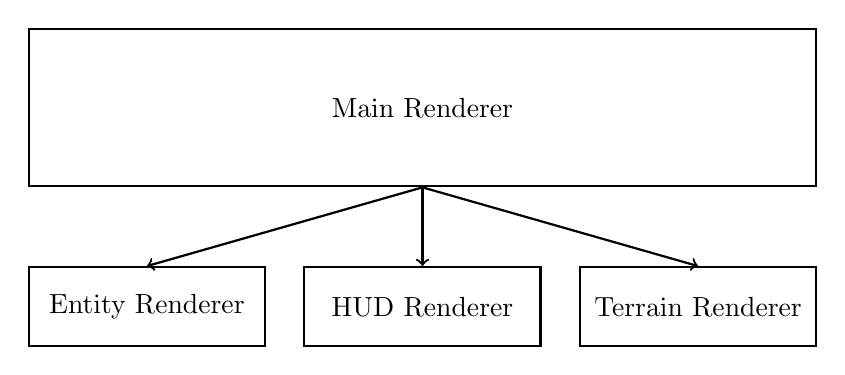
\begin{tikzpicture}
        % Main Renderer
        \node[draw, thick, minimum width=10cm, minimum height=2cm] (main) {Main Renderer};

        % Subrenderers: TerrainRenderer, HUDRenderer, EntityRenderer
        \node[draw, thick, minimum width=3cm, minimum height=1cm, below=1cm of main, xshift=-3.5cm] (entity) {Entity Renderer};
        \node[draw, thick, minimum width=3cm, minimum height=1cm, below=1cm of main] (hud) {HUD Renderer};
        \node[draw, thick, minimum width=3cm, minimum height=1cm, below=1cm of main, xshift=3.5cm] (terrain) {Terrain Renderer};

        % Arrows from main renderer to subrenderers
        \draw[->, thick] (main.south) -- (entity.north);
        \draw[->, thick] (main.south) -- (terrain.north);
        \draw[->, thick] (main.south) -- (hud.north);
    \end{tikzpicture}
\end{frame}

\begin{frame}{Rendering Architecture - Normal Mode}
    \centering
    \includegraphics[width=0.85\textwidth]{../figures/Ingame-Picture.png}
\end{frame}

\begin{frame}{Rendering Architecture}
    \begin{tabular}{ccc}

        \parbox{0.3\textwidth}{
            \centering \textbf{Entity Renderer}
            \vspace{0.2cm}
            \begin{itemize}
                \item Entities are rendered with their respective textures
                \item Handles animations of the entities, e.g. walking
            \end{itemize}
            \vspace{0.5cm}
            \centering
            \includegraphics[width=0.25\textwidth]{../../assets/texture/player_walk.png}
        } &

        \pause
        
        \parbox{0.3\textwidth}{
            \centering \textbf{Terrain Renderer}
            \vspace{0.2cm}
            \begin{itemize}
                \item Terrain is continuously rendered with a texture
            \end{itemize}
            \vspace{0.5cm}
            \centering
            \includegraphics[width=0.2\textwidth]{../../assets/layers/mountain3.png}
        } &

        \pause
        
        \parbox{0.3\textwidth}{
            \centering \textbf{HUD Renderer}
            \vspace{0.2cm}
            \begin{itemize}
                \item Heads-Up-Display (HUD) is rendered on top of the game
                \item Displays the player's health, score, inventory, etc.
            \end{itemize}
            \vspace{0.5cm}
            \centering
            \begin{tabular}{ccc}
                \includegraphics[width=0.07\textwidth]{../../assets/texture/coin.png} &
                \includegraphics[width=0.07\textwidth]{../../assets/texture/kaiserschmarrn.png} &
                \includegraphics[width=0.07\textwidth]{../../assets/texture/duck.png}
            \end{tabular}
        }
    \end{tabular}
\end{frame}




\begin{frame}{Rendering Architecture - Debug Mode}
    \centering
    \includegraphics[width=0.85\textwidth]{../figures/Debug-Mode.png}
\end{frame}
	\makesection{Conclusion}

\begin{frame}{Conclusion}

    \begin{itemize}
        \item Achievements:
        \begin{multicols}{4}
            \begin{tcolorbox}[colback=boxcolor, colframe=boxcolor, width=0.235\textwidth, height=4.5cm, rounded corners]
                \centering
                Modular and maintainable architecture and optimized codebase.
            \end{tcolorbox}
            
            \begin{tcolorbox}[colback=boxcolor, colframe=boxcolor, width=0.235\textwidth, height=4.5cm, rounded corners]
                \centering
                Design of a customizable physics engine which supports convex polygons.
            \end{tcolorbox}
            
            \begin{tcolorbox}[colback=boxcolor, colframe=boxcolor, width=0.235\textwidth, height=4.5cm, rounded corners]
                \centering
                Framework (based on OOP) that can be readily extended.
            \end{tcolorbox}
            
            \begin{tcolorbox}[colback=boxcolor, colframe=boxcolor, width=0.235\textwidth, height=4.5cm, rounded corners]
                \centering
                Enhanced user experience with new features (terrain, items, graphics..)
            \end{tcolorbox}
        \end{multicols}
        \item Tradeoff: OOP architecture is less performant than flecs.
    \end{itemize}
\end{frame}

\begin{frame}{Future Work}
    \begin{itemize}
        \item Multiplayer modes and leaderboard integration.
        \item New game items and biomes.
        \item Difficulty settings, coin shop to buy upgrades
        \item Further enhancements to the physics engine:
        \begin{itemize}
            \item Improved performance with parallel batch processing and spatial data structures.
            \item Friction and air resistance.
            \item Reduction of jitter.
        \end{itemize}
    \end{itemize}
    \centering
    \includegraphics[width = .5\textwidth]{../figures/physics/jitter.pdf}
\end{frame}

	
	%%%%%%%%%%%%%%%%%%%%%%%%%%%%%%%%%%%%%%%%%%%%%%%%%%%%%%%%%%%%%%%%%%%%%%%%%%%%%%%%
	%%%%%%%%%%%%%%%%%%%%%%%%%%%%%%%%%%%%%%%%%%%%%%%%%%%%%%%%%%%%%%%%%%%%%%%%%%%%%%%%

	\begin{frame}{Literatur}
		%\bibliographystyle{plain}%alpha, arabic
		%\bibliography{bib/literatur.bib}
		\AtNextBibliography{\tiny}
		\printbibliography
	\end{frame}

	%%%%%%%%%%%%%%%%%%%%%%%%%%%%%%%%% final slide %%%%%%%%%%%%%%%%%%%%%%%%%%%%%%%%%%
	\thankstotwo{Prof. Dr. M. Schulte}{C. Homs Pons, M.Sc.}{}
	\thankyou{survivingsarntal@gmail.com}{-}{-}
	
	%\thankstoone{Dirk Pflüger}{Something}
	%\thankstothree{Dirk Pflüger}{Dirk Pflüger}{Dirk Pflüger}{Something}
	%\thankstofour{Dirk Pflüger}{Dirk Pflüger}{Dirk Pflüger}{Dirk Pflüger}{Something}
	
\end{document}


%% Local Variables:
%% TeX-engine: luatex
%% End:
